% -*- coding: utf-8; -*-

\chapter{Processo de Restauração de Seções Geológicas}

\section{Sistema Recon MS}

\subsection{Introdução}

O ambiente no qual este trabalho é desenvolvido é o \textit{Sistema Recon MS}, um sistema computacional capaz de auxiliar no balanceamento de seções geológicas. Conta com editor gráfico, estruturas de dados topológicos, algoritmos de transformações geométricas, relatórios de pós-processamentos entre outros recursos.

O Recon MS é desenvolvido a partir de um convênio entre o Instituto Tecgraf/PUC-Rio e a Petrobras desde 1991.

Neste capítulo são apresentadas as principais características do Sistema Recon MS para o objeto deste trabalho a fim de prover uma contextualização para o que é exibido nos demais capítulos. As primeiras seções tratam da descrição dos recursos básicos usados pelo sistema no processo de restauração de seções geológicas. Ao fim, é mostrado a definição da linhas de mapeamento, bem como o tipo de mapeamento desenvolvido com base em tais linhas.

\subsection{Subdivisão Planar} % Falar do HED e da TopS

Uma seção geológica pode ter sua representação digital como uma subdivisão planar uma vez que ela pode ser vista como um conjunto de polígonos que dividem o domínio da seção. Estes polígonos podem sofrer deformações e deslocamentos oriundos das transformações geométricas às quais a seção pode sofrer durante o balanceamento. Há ainda informações de adjacências entres essas porções que também precisam ser consideradas em um contexto computacional da seção geológica.

Na Figura~\ref{fig-subdivisao-planar} é possível perceber, por exemplo, que as camadas A, B e C possuem 3 blocos separados por falhas. Cada bloco é uma região fechada delimitada por um conjunto de segmentos. Deve-se observar ainda que essas regiões possuem atributos geológicos como idade, litologia, porosidade, etc.

\begin{figure} [h]
  \begin{center}
    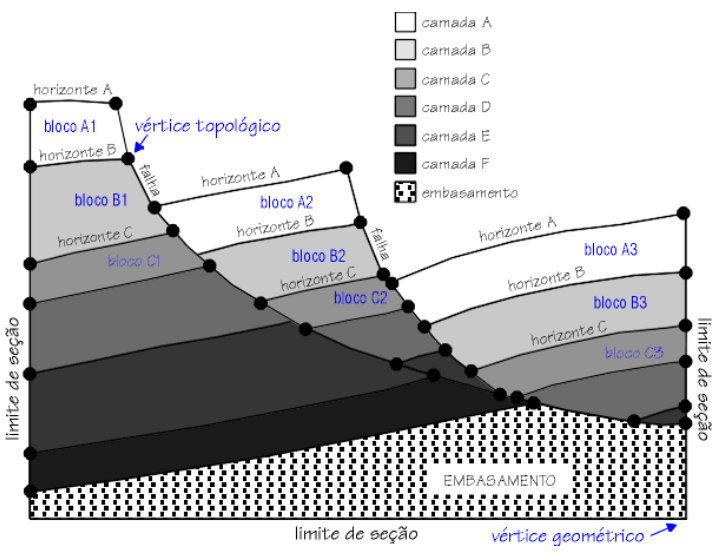
\includegraphics[width=400pt]{images/fig-subdivisao-planar}
    \caption{Seção geológica como uma subdivisão planar.\cite{Ferraz}}\label{fig-subdivisao-planar}
  \end{center}
\end{figure}

Uma subdivisão planar pode ser definida como uma subdivisão do plano através do uso de \textit{arestas}, \textit{vértices} e \textit{faces}. Essas são as entidades topológicas presentes em uma subdivisão planar, a face é como a região descrita anteriormente, delimitada por arestas (segmentos de curva); os vértices são os limites das arestas, sendo um para cada extremidade (podendo ser o mesmo vértice no início e no final da aresta).

A subdivisão planar precisa atender a alguns requisitos em relação às entidades topológicas: não deve haver vértices coincidentes; arestas só podem se cruzar em um vértice e faces também só se cruzam ou em um vértice, ou em uma aresta. Em outras palavras, não deve existir sobreposição de elementos topológicos. 

No entanto, há ainda um último componente topológico: o \textit{loop} ou \textit{laço} que é, de forma sucinta, um suconjunto conexo e ordenado de arestas. Com essa definição, a \textit{face} pode ser interpretada como uma união de laços, um deles sendo externo (delimitando a fronteira externa da face) e zero ou mais internos.

Em suma, a subdivisão planar tem os seguintes elementos topológicos:
\renewcommand{\labelitemi}{•}
\begin{itemize}
  \item \textbf{Vértice}: representa um ponto único dentro do plano.
  \item \textbf{Aresta}: segmento de curva com vértices como limites.
  \item \textbf{Laço} (loop): suconjunto conexo e ordenado de arestas.
  \item \textbf{Face}: região delimitada por um ou mais laços.
\end{itemize}

\subsection{Modelagem da Subdivisão Planar}

Para modelar a subdivisão planar dentro do Recon é utilizada a biblioteca computacional \textbf{HED} desenvolvida pelo Instituto Tecgraf/PUC-Rio. O HED é uma estrutura de dados topológica baseado em arestas, uma das razões para esta escolha são as relações fixas de adjacência que uma aresta apresenta em relação às outras componentes topológicas. Uma aresta sempre é delimitada por dois vértices (distintos ou não) e é adjacente à duas faces.

O HED introduz uma nova entidade que explora bem essa característica denominada \textit{half-edge} ou \textit{semiaresta} que é uma referência ao \quotes{uso} da aresta por uma face. Dessa forma, no HED, cada aresta é formada por duas semiarestas, cada semiaresta guarda uma referência para uma face e também para um vértice de origem. Isto dá uma orientação para a semiaresta que é usada para indicar o sentido positivo do loop das faces, por exemplo.

A estrutura HED tem um aspecto hierárquico de listas duplamente encadeada de elementos topológicos. No nível mais alto está a subdivisão planar, denominada como \textit{HedSolid}, então vêm \textit{HedFace}, \textit{HedLoop}, \textit{HedHalfEdge} e \textit{HedVtx} no nível mais baixo. A representação da aresta, \textit{HedEdge} encontra-se no mesmo nível da HedHalfEdge.

[ incluir uma tabela com as structs do HED ]

Uma propriedade importante em estruturas topológicas são as relações de adjacências entre suas componentes, a HED não provê de forma direta todos as relações, contudo é possível chegar às demais com uso de indireções. Por exemplo, partindo de uma aresta, como chegar às faces vizinhas? Basta ir às semiarestas da aresta, cada semiaresta possui referência para uma face.

Apresentado o HED e seus elementos, a associação com as entidades geológicas é intuitiva. Uma camada geológica é representada por uma face; as linhas de horizonte, falha ou sal têm como correspondente as arestas, por último, cada conjunto contínuo de faces é associado a um sólido\footnote{Os sólidos representam uma subdivisão planar e em alguns casos, a seção pode apresentar partes inteiramente descontínuas onde cada parte é um sólido.}.

Destaca-se que a ideia de representar a seção geológica como uma subdivisão planar, ou uma estrutura HED, visa facilitar a criação e manipulação computacional da seção durante o processo de restauração. Todavia, a representação completa precisa levar em consideração também os atributos geológicos.

\subsection{Atributos Geológicos}

Como já dito, os blocos que formam a seção geológica possuem propriedades próprias e precisam também estarem salvas na estrutura de dados topológica.

Cada entidade do HED possui um campo reservado para um tipo genérico de informações e é neste espaço que são organizados os atributos geológicos da seção. Estes atributos são representados em estruturas chamadas \textit{GeoSolid}, \textit{GeoFace}, \textit{GeoEdge} e \textit{GeoVtx}. Pela nomenclatura, é fácil observar a relação com o HED. As principais informações organizadas nessas estruturas são:

\renewcommand{\labelitemi}{•}
\begin{itemize}
  \item \textbf{GeoSolid}: o sólido por ser a estrutura mais alto nível, é quem vai guardar referência à seção e ao cenário ao qual pertence dentro da restauração.
  \item \textbf{GeoFace}: é a estrutura que precisa armazenar dados do material geológico que a compõe (como idade, tipo, características físicas, etc.) e malha de triângulos que pode ser manipulada pelas transformações.
  \item \textbf{GeoEdge}: estrutura que guarda o tipo de linha (de horizonte, falha, topo de sal, etc.) e a subdivisão geométrica que forma a linha. 
  \item \textbf{GeoVtx}: é a única que armazena apenas o identificador universal.
\end{itemize}

Aliás, todas as estruturas de atributos geológicos possuem um campo para salvar este identificador no formato de um \textit{UUID} --- \textit{universally unique identifier}\cite{UUID} ou identificador único universal que é usado, por exemplo, na associação dos elementos geológicos com a malha triangular das faces, que será apresentada adiante.

\subsection{Seções Geológicas} % Falar da árvore de cenários



%\section{Estruturas Geológicas}

%\subsection{Comportamento dos Materiais e Rochas}

%\subsection{Seções Geológicas}

%\section{Restauração de Seções Geológicas}

%\subsection{Sistema Recon MS}


